\documentclass[twoside,12pt,a4paper]{scrreprt}
\usepackage[T1]{fontenc}
\usepackage[utf8]{inputenc}
\usepackage[ngerman]{babel}
\usepackage{babelbib}
\usepackage{parskip}
\usepackage{microtype}
\usepackage{graphicx} % Zum Einbinden von Grafiken
\usepackage[dvipsnames]{xcolor}
\usepackage[colorlinks=true,linkcolor=Black,citecolor=MidnightBlue,urlcolor=MidnightBlue]{hyperref}
\usepackage[all]{hypcap}
\usepackage{pgfplots} \pgfplotsset{compat=1.9}
\usepackage{helvet} % Schönere SansSerif-Schrift
\usepackage{times}  % Schönere Serif-Schrift

\usepackage{blindtext} % sollte am Ende nicht mehr benötigt werden ;)

\pagestyle{headings}

\graphicspath{ {figures/} } % Pfad-Prefix für einzubindende Grafiken. Es sind auch mehrere Pfade möglich, diese müssen jeweils in eigenen {Klammern} stehen.

\setkomafont{disposition}{\normalcolor\bfseries} % überall Serifen verwenden
% oder
%\renewcommand{\familydefault}{\sfdefault} % überall Sans-Serif verwenden

% PDF-Optionen (werden in den Dateieigenschaften angezeigt)
\hypersetup{
pdftitle={Titel der Arbeit},
pdfauthor={Vor- und Nachname},
pdfsubject={Bachelorarbeit Informatik},
pdfpagelayout=TwoColumnRight
}

%%% Eigene Makros
\newcommand{\qq}[1]{\glqq #1\grqq} % \qq{Text in Anführungszeichen}

\begin{document}

%%% Titelseite
\begin{titlepage}
\begin{center}
\LARGE Eberhard Karls Universität Tübingen\\
\large Mathematisch-Naturwissenschaftliche Fakultät \\
Wilhelm-Schickard-Institut für Informatik\\
[3cm]
\huge Bachelorarbeit Informatik\\
[2cm]
\Large\textbf{Titel der Arbeit (der geht wohl in den\\ meisten Fällen über mehr als eine Zeile)}\\
[1.5cm]
\large Vor- und Nachname\\
[0.5cm]
Datum\\
\vfill
\small\textbf{Gutachter}\\[0.3cm]
\large Name Gutachter\\
\footnotesize Wilhelm-Schickard-Institut für Informatik\\Universität Tübingen\\
[1cm]
\small\textbf{Betreuer}\\[0.3cm]
\large Name Betreuer\\
\footnotesize Adresse\\
Universität Tübingen
\end{center}
\end{titlepage}

%%% Titelrückseite: Bibliographische Angaben
\thispagestyle{empty}
\vspace*{\fill}
\textbf{Nachname, Vorname:}\\
\emph{Titel der Arbeit}\\
Bachelorarbeit Informatik\\
Eberhard Karls Universität Tübingen\\
Bearbeitungszeitraum: Anfangs- -- Enddatum
\newpage

%%% Zusammenfassung (Abstract), hier aus externer Datei eingebunden
\begin{abstract}
\section*{Zusammenfassung}
Das hier entwickelte Kommandozeilenprogramm extrahiert Bilder aus einer eingescannten Fotoalbumseite und kann Gesichter detektieren. Zum extrahieren wird der Floodfill-Algorithmus verwendet, der anhand der Hintergrundfarbe des Fotoalbums die Bilder ausschneidet. Um noch einen vorhandene Rahmen zu entfernen werden die Kanten des Bildes mit dem Canny-Algorithmus detektiert und an den Seiten des Bildes nach einem Bereich gesucht an dem keine Kanten sind. Danach kann mit Hilfe eines Cascade Classifier Gesichter in den Bildern detektiert werden. Dies geschieht sowohl für Gesichter im Profil als auch für Gesichter die direkt in die Kamera schauen. Um die Ergebnisse zu überprüfen werden die Bilder auf Größe, Featureposition und Strukturelle Ähnlichkeit hin überprüft. Das Programm arbeitet sehr gut bei Bildern mit einem deutlichen Rahmen und die gerade in der Seite ausgerichtet sind. Bilder deren Farbwerte stark dem Hintergrund ähneln oder die sich schräg in dem Fotoalbum befinden werden schlecht ausgeschnitten. Für die Gesichtserkennung ist die Qualität und Auflösung der Bilder ausschlaggebend. Bei schlechter Qualität werden wesentlich weniger Gesichter erkannt als bei Bilder mit guter Qualität.
\end{abstract}
\newpage

%%% Inhaltsverzeichnis
\KOMAoption{toc}{listof,bib} % Abbildungs-/Tabellenverzeichnis, Literaturverzeichnis aufnehmen
\tableofcontents\label{toc}
\cleardoublepage

%%% Hauptteil (mit \input{dateiname} wird die Datei 'dateiname' eingebunden)
\chapter{Einleitung}

% problemstellung
% ziele definieren
% vorhandene daten beschreiben
\section{Problemstellung}

\section{Benutzte Technologien}
% genutzte methoden, toolboxen, programmiersprachen

\section{Programmaufbau}

\cleardoublepage

% !TEX root = ../ausarbeitung.tex

\chapter{Stand der Forschung}
Hier zeigen Sie, dass Sie über Ihr Themengebiet gut informiert sind. Sie können entweder den Stand der Forschung dafür heranziehen, um Ihr Thema zu rechtfertigen (\qq{Warum ist es wichtig?}) oder Sie können die Literatur als Grundlage Ihrer Diskussion verwenden (Wie ordnen sich Ihre Beiträge in die Wissenschaftslandschaft allgemein ein?), eine Mischung ist auch möglich.

\hfil\rule{0.4\textwidth}{0.4pt}

Dazu gehören natürlich Referenzen zu anderen Werken. Für deren Verwaltung empfiehlt sich BibTeX, die entsprechende Datei \verb|literatur.bib| (kann natürlich auch anders benannt sein) ist in der Vorlage schon enthalten. Zur Einhaltung der Syntax bietet sich ein Online-Editor wie \cite{BibTexOnlineEditor} an; TeXstudio \cite{texstudio} hält im Menü auch Hilfe beim Erstellen der Bibliographie-Einträge bereit. Für Bücher bietet z.B. auch \url{https://books.google.de/} fertige BibTeX-Einträge an.

Die Einbindung in den Text erfolgt dann mit \verb|\cite{nielsen1994usability}|, wobei der Text in den Klammern durch das in der \verb|.bib|-Datei vergebene Kürzel ersetzt werden müssen. Das Ergebnis ist dann eine Referenz zum (zumindest im Bereich \qq{Usability Engineering}) fast unverzichtbaren gleichnamigen Buch \cite{nielsen1994usability} von Jakob Nielsen.

Achtung: Ihre Ausarbeitung sollte sich (im Gegensatz zu diesem Template) weniger auf Internet-Quellen, als auf Bücher und Paper stützen!
\\

\Blindtext[5]
\cleardoublepage

% !TEX root = ../ausarbeitung.tex

\chapter{Herangehensweise}

Im Hauptteil beschreiben Sie Ihre praktische Arbeit. Code gehört normalerweise nicht in eine Ausarbeitung. Ausnahmen sind Algorithmen, die für Sie wichtig waren (dann in möglichst übersichtlichem Pseudo-Code). Kleine Code-Stücke können auch zur Illustration oder als Beispiel eingebaut werden. Längere Code-Stücke können im Anhang untergebracht werden. Sie sollten jedoch nicht den gesamten Code im Anhang abdrucken. Ihren Code geben Sie bitte dennoch mit ab, am besten auf einer CD.

Der Detailgrad sollte so sein, dass ein Leser die gleiche Arbeit noch einmal nachimplementieren könnte. Insbesondere sollten alle Parameter, von denen die Funktionsweise des Systems abhängt, explizit genannt sein. Bei der Evaluation muss bei jedem Versuch angegeben werden, mit welchen Parametern gearbeitet wird.


\hfil\rule{0.4\textwidth}{0.4pt}

\section{Einführung in \LaTeX}
Wenn Sie dieses Template gefunden haben, werden Sie schon erkannt haben, dass \LaTeX\ nicht ganz unwichtig ist. Falls Sie noch kaum oder keine Erfahrung damit haben, bietet sich der Kurs \qq{Einführung in \LaTeX} von Thorsten Nagel an. Er findet meistens mehrmals im Semester statt, die genauen Termine entnehmen Sie bitte dem Vorlesungsverzeichnis. Das Skript zu diesem Kurs ist online erhältlich \cite{thorstennagel2015} und enthält noch viele weitere Informationen, die in der folgenden Kurzzusammenfassung nicht berücksichtigt werden konnten.

\section{Sinnvolle Programme}
Falls Sie \verb|.tex|-Dateien nicht unbedingt in einem normalen Texteditor schreiben und auf der Kommandozeile kompilieren möchten, bietet sich ein spezieller \LaTeX-Editor wie z.B. TeXstudio \cite{texstudio} an.

\section{Wichtige \LaTeX-Befehle}
\subsection{Textgliederung}
Mit dem Befehl \verb|\section{Überschrift}| lässt sich ein neuer Abschnitt beginnen, der automatisch nummeriert und im \hyperref[toc]{Inhaltsverzeichnis} eingetragen wird.
Gleiches gilt für einen Unterabschnitt, der mit \verb|\subsection{Unterüberschrift}| begonnen wird.

\LaTeX\ bietet noch weitere Gliederungsebenen bis hin zum Unterabsatz, die aber standardmäßig nicht mehr nummeriert werden und standardmäßig auch nicht im Inhaltsverzeichnis auftauchen. Im Normalfall sind diese aber nicht unbedingt nötig.
\subsubsection{Unterunterüberschrift}
\paragraph{Absatztitel} Absatztext
\subparagraph{Unterabsatz} Absatztext

Um in der PDF-Datei einen Zeilenumbruch zu erhalten, schreiben Sie im Quelltext \verb|\\|, für einen neuen Absatz lassen Sie eine Zeile frei. Ein einzelner Zeilenumbruch im Quelltext hat keine Auswirkungen.

\section{Formatierungen, Listen, Aufzählungen}
Um die \LaTeX-Befehle für die folgenden Formatierungen zu sehen, schauen Sie sich einfach den Quellcode an.

Text kann man \textbf{fett} oder \textit{kursiv} schreiben. Sie können Text auch explizit \emph{betonen}, was dann ebenfalls kursiv dargestellt wird.

Listen sind natürlich auch möglich, diese können beliebig verschachtelt werden.
\begin{itemize}
\item Listenpunkt 1
\item Listenpunkt 2
\begin{itemize}
\item Unterpunkt
\end{itemize}
\end{itemize}

Oder eine nummerierte Aufzählung:
\begin{enumerate}
\item Listenpunkt 1
\item Listenpunkt 2
\begin{enumerate}
\item Unterpunkt
\end{enumerate}
\end{enumerate}

\section{Tabellen}
Tabellen können wie folgt erstellt werden (siehe \autoref{tab:tabelle-1}):
\begin{table}[htb]
\centering
\caption{Formatierungsparameter zur Spaltenausrichtung in Tabellen\label{tab:tabelle-1}}
\begin{tabular}{l|p{3.5cm}lcr}
	                     & \textbf{Spalte 1}                   & \textbf{Spalte 2} & \textbf{Spalte 3} & \textbf{Spalte 4} \\ \hline
	\textbf{Parameter}   & \verb|p{3.5cm}|                     & \verb|l|          &     \verb|c|      &          \verb|r| \\
	\textbf{Ausrichtung} & linksbündig mit vorgegebener Breite & linksbündig       &     zentriert     &      rechtsbündig
\end{tabular}
\end{table}

Für \qq{schönere} Tabellen empfiehlt sich das \LaTeX-Paket \verb|booktabs|, das in der Präambel mit \verb|\usepackage{booktabs}| eingebunden werden kann. Insbesondere die zugehörige Anleitung \cite{booktabs} ist lesenswert, da sie recht einfach vermittelt, was eine \qq{schöne} Tabelle ausmacht.

\section{Mathematische Gleichungen}
Gleichungen oder sonstige Formeln im Fließtext, wie z.B. $f(x)=ax+b$, können Sie einfach in Dollarzeichen \verb|$...$| einfassen. Größere Formeln können auch in einer eigenen Zeile stehen:
\begin{displaymath}
g(x) = \frac{1}{2\pi\sigma}\cdot e^{-\frac{(x-\mu)^2}{2\sigma^2}}
\end{displaymath}
Falls Sie in Ihrer Ausarbeitung viel Mathematik benötigen, lohnt sich auch ein Blick auf das \LaTeX-Paket \verb|amsmath|.
\section{Abbildungen}
Abbildungen und Diagramme können Sie direkt in einer \verb|.tex|-Datei \qq{malen}. Dazu bietet TikZ viele Möglichkeiten, eine Grafik mit Text zu beschreiben. Falls Sie nicht jeden Strich in einem Diagramm selbst definieren wollen, bietet sich die Verwendung von Pgfplots in Form der \verb|axis|-Umgebung an, wie in \autoref{fig:diagramm} gezeigt.

Falls Sie sich näher mit der Materie beschäftigen wollen, bietet sich das Manual für TikZ und PGF\cite{pgfmanual} an. Dieses Dokument ist zwar sehr umfangreich (über 1000 Seiten), bietet aber viele gut erklärte Beispiele, auch und gerade für den Einstieg.

Die folgenden Abbildungen wurden in jeweils eine \verb|figure|-Umgebung gesteckt. Diese erzeugt eine \qq{floatende} Abbildung, die von \LaTeX\ automatisch an einer \qq{geeigneten} Stelle platziert wird, also nicht zwangsläufig dort, wo sie im Quelltext definiert wurde. Wenn Sie der Abbildung eine \verb|\caption{...}| und ein \verb|\label{key}| verpassen, können Sie über dieses Label im Text per \verb|\ref{key}| oder \verb|\autoref{key}| darauf verweisen. Bei ersterem wird nur die Nummer (\qq{\ref{fig:diagramm}}), bei letzterem zusätzlich noch der Typ (\qq{\autoref{fig:diagramm}}) ausgegeben. Analog zur \verb|figure|-Umgebung wurde oben für die Tabelle die \verb|table|-Umgebung verwendet.
\begin{figure}[htb]
\centering
\begin{tikzpicture}
  \begin{axis}[xlabel=$x$,ylabel=$y$,width=0.75\textwidth]
    \addplot[smooth,mark=*,blue] plot coordinates {
        (0,2)
        (2,3)
        (3,1)
    };
    \addlegendentry{Case 1}

    \addplot[smooth,color=red,mark=x] plot coordinates {
            (0,0)
            (1,1)
            (2,1)
            (3,2)
        };
    \addlegendentry{Case 2}
  \end{axis}
\end{tikzpicture}
\caption{Diagramm aus den TikZ-Beispielen für Pgfplots\label{fig:diagramm}}
\end{figure}

Falls Sie eine Abbildung schon als separate Datei (z.B. im PDF-Format) vorliegen haben, können Sie diese mit \verb|\includegraphics{}| und dem Dateinamen einbinden, wie in \autoref{fig:smileys} geschehen. Dabei wird in den in der Präambel mit \verb|\graphicspath{...}| vorgegebenen Pfaden gesucht. Die Dateiendung wird automatisch \qq{erraten}, wenn sie nicht angegeben wird.
\begin{figure}[htb]
	\centering
	
\includegraphics[width=0.75\textwidth]{smileys}
	\caption{Darstellung des Wohlbefindens anhand von Smileys\label{fig:smileys}}
\end{figure}

\cleardoublepage

\chapter{Auswertung}

\section{Metriken zur Auswertung}
\subsection{Bildgröße}
Da es in dem Projekt um das Ausschneiden von Bildern geht ist die Bildgröße eine nahe liegende Metrik um die Genauigkeit unserer Software zu messen. Die Größe wird berechnet indem die Höhe mit der Breite multipliziert wird. Von der so ermittelten Größe des ausgeschnittenen Bildes wird die Größe des Ground Truth Bildes abgezogen. Aus dieser Differenz wird der Prozentuale unterschied zum Ground Truth Bild berechnet. Sollte das Ergebnis negativ sein ist das ausgeschnittene Bild kleiner als der Ground Truth.
   
\subsection{Bildmerkmale}
Eine weitere Metrik ist das erkennen gleicher Bildmerkmale. Dazu wird der patent freie ORB (Orientatet FAST and Rotated BRIEF) detektor von OpenCV verwendet der Rotations invariant ist. ORB ist eine fusion zwischen dem FAST Schlüsselpunkt Detektor and BRIEF Beschreibung der Schlüsselpunkte mit vielen Modifikationen um die Geschwindigkeit des Algorithmus zu verbessern (\cite{OpenCVORB}). Die so erkannten Merkmale werden dann der reihe nach anhand der Distanz zum Bildzentrum verglichen. Es wird für jedes erkannte Bildmerkmal die Distanz zum Zentrum des dazu gehörigen Bildes berechnet und das dann mit den Ergebnissen des Ground Truth verglichen. Solange zwischen den beiden Merkmalen keine zu großer Unterschied in der Distanz ist werden sie als gleich angesehen. Durch dieses Verfahren kann erkannt werden das sich der Ausschnitt des ausgeschnittenen Bildes an der selben stelle befindet, wie der Ground Truth und nicht nur die gleiche Größe ausgeschnitten wurde.

\subsection{Struktureller Ähnlichkeit (SSIM)}
Um ein Bild auf Gleichheit zu untersuchen verwenden wir den Strukturellen Ähnlichkeitsindex (Structural Similarity index, SSIM). Dieser berechnet die Ähnlichkeit zwischen verschiedenen Bildausschnitten mit folgender Gleichung:
$$
SSIM(x,y) = \frac{(2 \mu_x \mu_y + c_1)(\sigma_{xy} + c_2)}{(\mu^2_x + \mu^2_y + c_1)(\sigma^2_x + \sigma^2_y + c_2)}
$$ 
mit $\mu$ als Durchschnitt und $\sigma$ als Varianz bzw. Kovarianzmatrix des Bildausschnittes. $c$ sind da um die Division zu stabilisieren (\cite{Wang2004}). Das Verfahren lässt sich nur auf gleich große Bilder anwenden. Aus diesem Grund verkleinern wir die Bilder mit einer linearen Interpolation auf eine Größe von 64 x 64 Pixeln. Auf die so verkleinerten Bilder wird dann der SSIM angewandt. Um so näher das Ergebnis an 1 ist um so ähnlicher sind die beiden Bilder. 

\section{Ausgeschnittene Bilder}
In der Tabelle \ref{tab:metrics} sind die Ergebnisse für einige der Testbilder dargestellte den direkten Vergleich kann man in Abbildung ?? sehen dort sind die Bilder nebeneinander aufgezeigt. 

\begin{table}[h]
	\centering
	\begin{tabular}{c|ccc}
	Bild & Größe & Merkmale & SSIM \\ \hline 
	01 & 1.92 & 3.64 & 0.82 \\
	02 & 1.60 & 2.39 & 0.77 \\
	03 & -5.52 & 10.12 & 0.36 \\
	04 & 3.15 & 16.54 & 0.68 \\ 
	05 & 1.48 & 2.65 & 0.81 \\ \hline
	06 & -4.42 & 23.58 & 0.55 \\ 
	07 & 2.96 & 4.40 & 0.80 \\
	08 & 8.82 & 8.07 & 0.39 \\
	09 & -1.24 & 2.06 & 0.70 \\
	10 & -0.58 & 5.57 & 0.76 \\ \hline
	11 & -4.35 & 28.46 & 0.49 \\
	12 & 2.96 & 1.74 & 0.80 \\
	13 & 1.26 & 3.24 & 0.88 \\
	14 & 3.01 & 1.94 & 0.72 \\
	15 & 0.76 & 19.51 & 0.60 
	\end{tabular}
	\caption{Ergebnisse der Vergleichsmetriken der ausgeschnittenen Bilder.}
	\label{tab:metrics}
\end{table}


\section{Gesichtserkennung}
Die von OpenCV mitgelieferten Methoden zur Gesichtserkennung auf Bildern funktioniert grundsätzlich gut. Sie ist einfach anwendbar, hat eine vertretbare Laufzeit (der Algorithmus läuft nur einige Sekunden auf einer ganzen eingescannten Albumseite) und erkennt zumindest einen Großteil der Gesichter in den Fotos. \\
Um die Performanz der Classifier einzeln und in Kombination auszuwerten, wurden Wahrheitsmatrizen aufgestellt. Ausgewertet werden jeweils die korrekt erkannten Gesichter (True Positives (TP): positive - positive), die nicht erkannten Gesichter (False Negatives (FN): positive - negative) und die fälschlicherweise erkannten Gesichter (False Positives (FP): negative - positive). Korrekt nicht erkannte Gesichter (True Negatives (TN): negative - negative) gibt es in unserem Anwendungsfall nicht.\\
Tabellen \ref{tab:set1frontal} und \ref{tab:set2frontal} zeigen die Metriken in dem ersten und dem zweiten Datensatz wenn nur der frontal faces Classifier angewendet wird. Die daraus errechnete Genauigkeit \footnote{Formel für die Berechnung der Genauigkeit (\grqq Accuracy\grqq) ist: $\frac{TP + TN}{TP + FN + TN + FP}$, ($TN = 0$ in unserem Fall).} beträgt im ersten Datensatz 0.75 und im zweiten 0.59.\\
\begin{table}[h]
	\centering
	\begin{tabular}{l|lll}
		\hline
		& \multicolumn{3}{l}{Reference} \\ \hline
		\multirow{3}{*}{Prediction} &  & Positive & Negative \\
		& Positive & 270 & 1 \\
		& Negative & 88 & - \\ \hline 
	\end{tabular}
	\caption{Wahrheitsmatrix im ersten Datensatz, wenn nur der frontal-Classifier zum Einsatz kommt. Die Genauigkeit der Gesichtserkennung beträgt 0.75.}
	\label{tab:set1frontal}
\end{table}
\begin{table}[h]
	\centering
	\begin{tabular}{llll}
		\hline
		& \multicolumn{3}{l}{Reference} \\ \hline
		\multirow{3}{*}{Prediction} &  & Positive & Negative \\
		& Positive & 282 & 7 \\
		& Negative & 172 & - \\ \cline{2-4} 
	\end{tabular}
	\caption{Wahrheitsmatrix im zweiten Datensatz, wenn nur der frontal-Classifier zum Einsatz kommt. Die Genauigkeit der Gesichtserkennung beträgt 0.59.}
	\label{tab:set2frontal}
\end{table}
Wenn der zweite Classifier zur Erkennung von Profilen mit dazu genommen wird, erhöht sich die Anzahl der erkannten Gesichtern ein wenig. Das ist in Tabellen \ref{tab:set1frontalprofile} und \ref{tab:set2frontalprofile} zu sehen. Die Gesichter, die bereits von dem frontal-Classifier erkannt wurden, werden automatisch heraus gefiltert. Danach bleibt ein kleiner Mehrgewinn durch die Anwendung des profile-Classifiers übrig, die Performanz verbessert sich auf 0.76 und 0.65 jeweils.
\begin{table}[h]
	\centering
	\begin{tabular}{llll}
		\hline
		& \multicolumn{3}{l}{Reference} \\ \hline
		\multirow{3}{*}{Prediction} &  & Positive & Negative \\
		& Positive & 274 & 2 \\
		& Negative & 84 & - \\ \cline{2-4} 
	\end{tabular}
	\caption{Wahrheitsmatrix im ersten Datensatz, wenn frontal- und profile-Classifier kombiniert werden. Die Genauigkeit der Gesichtserkennung beträgt 0.76.}
	\label{tab:set1frontalprofile}
\end{table}
\begin{table}[h]
	\centering
	\begin{tabular}{llll}
		\hline
		& \multicolumn{3}{l}{Reference} \\ \hline
		\multirow{3}{*}{Prediction} &  & Positive & Negative \\
		& Positive & 301 & 8 \\
		& Negative & 153 & - \\ \cline{2-4} 
	\end{tabular}
	\caption{Wahrheitsmatrix im zweiten Datensatz, wenn frontal- und profile-Classifier kombiniert werden. Die Genauigkeit der Gesichtserkennung beträgt 0.65.}
	\label{tab:set2frontalprofile}
\end{table}

\subsubsection*{Festlegung der Ground Truth}
Die Referenz für die Auswertung der Gesichtserkennung festzulegen ist nicht trivial. Auf den alten Fotos sind aufgrund der schlechten Qualität der Aufnahmen viele Gesichter nicht tatsächlich zu erkennen. Vielmehr erschließt sich ein menschlicher Betrachter aus dem Kontext die Information, dass sich an gewissen Stellen ein Gesicht befinden muss. Das wurde bei der Festlegung der Ground Truth berücksichtigt. So wurden beispielsweise besonders kleine, verdeckte oder stark verschwommene Gesichter für die Berechnung der Metriken nicht berücksichtigt. Die Classifier haben außerdem Probleme, Gesichter zu erkennen, wenn starke Okklusionen auftreten, selbst wenn das Gesicht nur im Profil zu erkennen ist oder die Person eine Kopfbedeckung trägt. Diese wiederum wurden in die Gesamtsumme der Gesichter mit einberechnet. Im Folgenden werden exemplarisch einige Bilder gezeigt, die der Gesichtserkennungsalgorithmus nicht erkennen kann und die deswegen nicht in die Auswertung mit einbezogen wurden.\\
Bild \ref{fig:neg_ex1} zeigt ein kleines Mädchen, jedoch ist die Aufnahme sehr verschwommen. Jeder Mensch, der das Bild betrachtet, weiß, dass das Mädchen ein Gesicht haben muss. Wenn jedoch die Kontextinformationen entfernt werden würde, wäre es selbst für einen Menschen schwer, ein Gesicht zu identifizieren.\\
\begin{figure}[h]
	\centering
	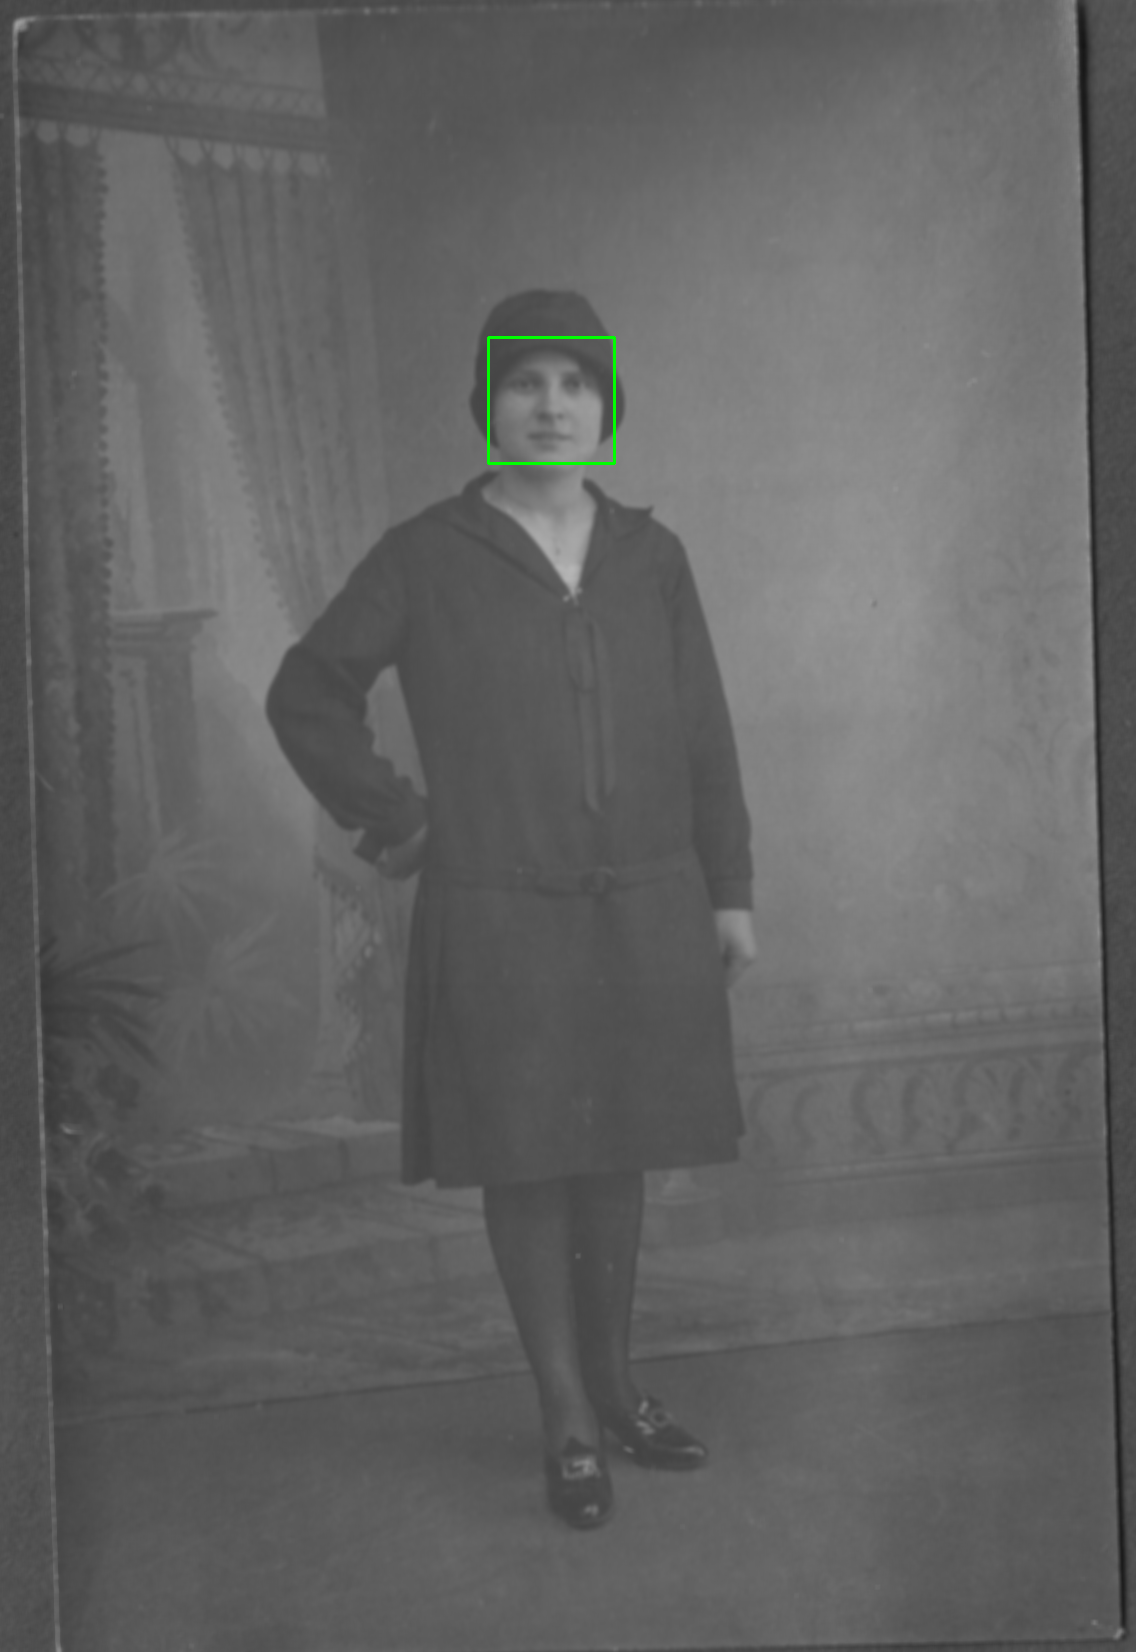
\includegraphics[width=0.75\linewidth]{images/examples_groundtruth/negative/04_1.png}
	\caption{Starke Bewegung im Bild verhindert, dass das Gesicht des Mädchens tatsächlich zu sehen ist, auch wenn menschliche Betrachter durchaus ihr Gesicht erkennen könnten.}
	\label{fig:neg_ex1}
\end{figure}
Auf Bild \ref{fig:neg_ex2} ist eine ähnliche Situationen zu sehen: alle abgebildeten Menschen haben Gesichter, jedoch sind sie objektiv nicht wirklich zu sehen. Sie sind relativ klein, was normalerweise für den Classifier kein Problem darstellt, aber eine schlechte Beleuchtung und geringer Kontrast tragen dazu bei, dass die Gesichter nicht erkannt werden.\\
\begin{figure}[h]
	\centering
	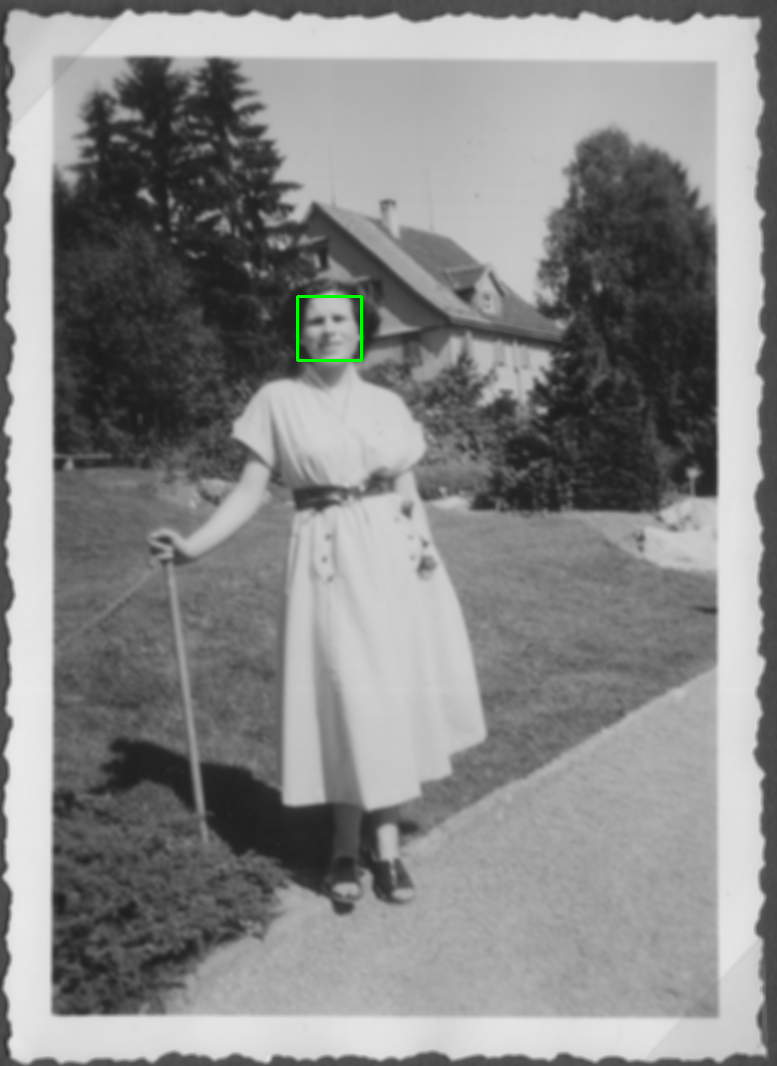
\includegraphics[width=0.75\linewidth]{images/examples_groundtruth/negative/29_2.png}
	\caption{Die Gesichtserkennung schlägt fehlt, wenn die Gesichter zu schlecht beleuchtet sind und/oder zu wenig Kontrast aufweisen. Auch, wenn normalerweise auch Gesichter in dieser Größe von dem Algorithmus problemlos erkannt werden.}
	\label{fig:neg_ex2}
\end{figure}
Um dennoch eine repräsentative Auswertung der Performanz der Gesichtserkennung zu gewährleisten, wurden viele nicht erkannte Gesichter mit in die Metriken einberechnet. Beispielsweise können die Classifier keine Gesichter mit Kopfbedeckungen erkennen. Ansonsten sind aber die Gesichter gut zu identifizieren, was in Bild \ref{fig:pos_ex1} zu sehen ist.\\
\begin{figure}[h]
	\centering
	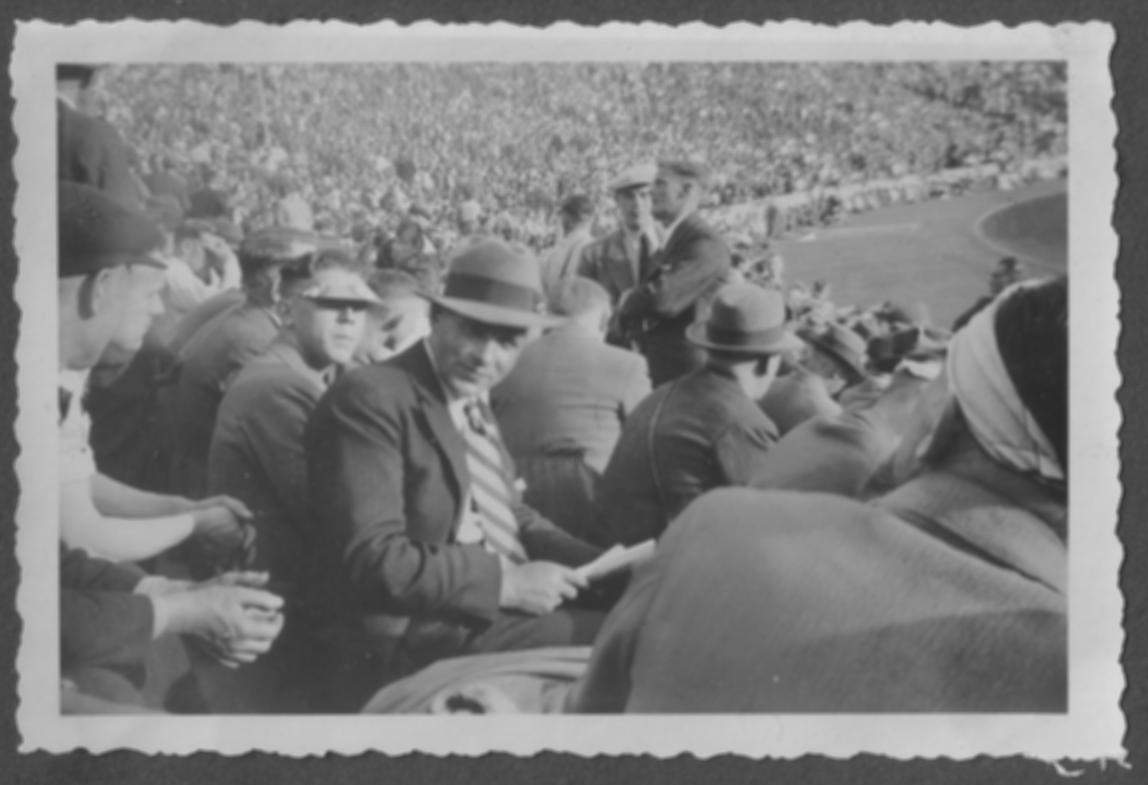
\includegraphics[width=0.75\linewidth]{images/examples_groundtruth/positive/32_3.png}
	\caption{Kein Classifier erkennt Gesichter mit Hüten, auch wenn sie nur einen kleinen Teil vom Gesicht verdecken. Alle anderen Gesichter werden problemlos identifiziert.}
	\label{fig:pos_ex1}
\end{figure}
Bild \ref{fig:pos_ex2} zeigt einen problematischen Grenzfall aus dem zweiten Datensatz. In diesem Bild wurden insgesamt drei Gesichter erkannt (zwei vom frontal-Classifier (grün) und eins vom profile-Classifier (rot)). Da alle Gesichter in etwa die gleiche Größe und Schärfe haben, sollte angenommen werden, dass auch die restlichen Personen erkannt werden. Es ist nicht ersichtlich, warum auf diesem Bild beide Classifier keine weiteren Gesichter erkennen. Von daher fließen alle Gesichter auf diesem Foto mit in die Bewertung ein und erhöhen die Anzahl der False Negatives enorm. Besonders im zweiten Datensatz kommen solche Fälle häufiger vor, was die schlechte Performanz des Algorithmus' im Vergleich zum ersten Datensatz erklärt.
\begin{figure}[h]
	\centering
	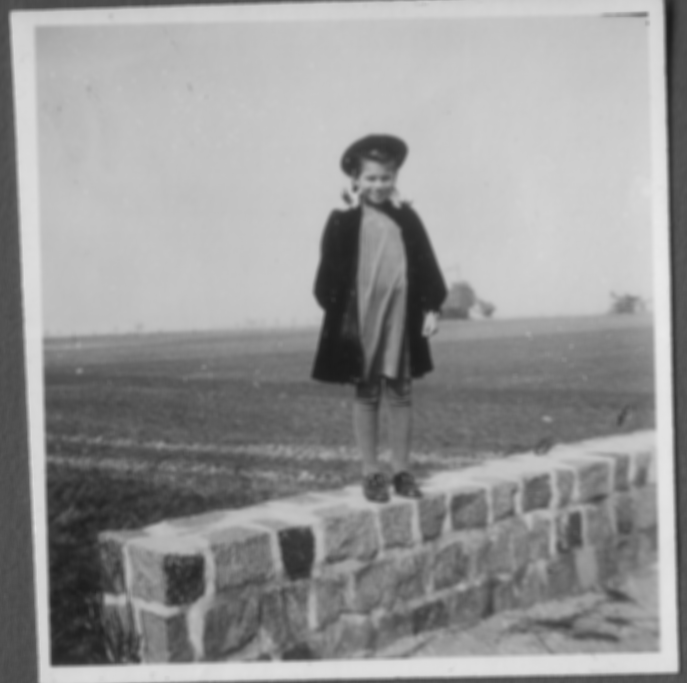
\includegraphics[width=0.75\linewidth]{images/examples_groundtruth/positive/16_1.png}
	\caption{In diesem Gruppenfoto werden nur wenige Gesichter erkannt, obwohl sie alle ähnlich aussehen. Das verschlechtert die Kennwerte für die Genauigkeit besonders im zweiten Datensatz stark.}
	\label{fig:pos_ex2}
\end{figure}
\cleardoublepage

% !TEX root = ../ausarbeitung.tex

\chapter{Diskussion}
Die Diskussion kann als Teil des Evaluations- oder Schlusskapitels oder als eigenständiges Kapitel aufgeführt werden. Wichtig ist, dass Sie Ihre Evaluationsergebnisse realistisch einschätzen und ins Verhältnis zum Stand der Technik setzen. Achten Sie besonders darauf, aus den Daten Ihrer Evaluation keine Wunschergebnisse abzulesen, die nicht in den Daten sind (wenn Ihre Testnutzer Ihr neuimplementiertes System nicht besser bedienen können als ein vorhandenes, dann ist das eben so). Gerade unerwartete bzw. \qq{negative} Ergebnisse (z.B. das neue System ist nicht besser als vorhandene) bringen wissenschaftliche Erkenntnisse: man stellt damit fest, dass der gewählte Weg nicht zum gewünschten Ergebnis führt und man generiert damit neue Fragen, z.B. warum der Weg nicht funktioniert hat, obwohl er vor dem Test als überlegen erachtet wurde.

Es kann auch sein, dass verschiedene Evaluationsformen Unterschiede offenbaren. Z.B. kann es sein, dass die Nutzbarkeit des implementierten Systems nicht besser ist als bei anderen Ansätzen, aber dass es deutlich einfacher zu warten ist.


Im letzten Teil runden Sie Ihre Arbeit ab, in dem Sie Ihre Argumentation aus der Einleitung aufgreifen und mit konkreten Daten aus Ihrem Hauptteil und der Evaluation untermauern. Auch hier können Sie Bezug zur Literatur nehmen. Am Ende sollten Sie einen Ausblick über weitere Forschungsthemen geben. Dabei aufpassen, dass es nicht so klingt wie \qq{mir ist die Zeit ausgegangen und folgendes habe ich nicht mehr geschafft}. Eine gute wissenschaftliche Arbeit wirft mehr Fragen auf als sie beantwortet. Es sollte also eher klingen nach \qq{meine Arbeit hat \dots gezeigt. Daraus ergeben sich weitere interessante Fragen \dots}.
\cleardoublepage

%%% Literaturverzeichnis, lädt die Datei literatur.bib
\bibliographystyle{babplain} % "babplain" benötigt das Paket babelbib
\bibliography{literatur}
\cleardoublepage

%%% Selbständigkeitserklärung
\thispagestyle{empty}
\section*{Erklärung}
Hiermit erkläre ich, dass ich diese schriftliche Abschlussarbeit selbständig 
verfasst habe, keine anderen als die angegebenen Hilfsmittel und Quellen benutzt 
habe und alle wörtlich oder sinngemäß aus anderen Werken übernommenen Aussagen als 
solche gekennzeichnet habe.
\\[2cm]
Ort, Datum \hfil Unterschrift 

\end{document}